% \chapter{Instandhaltung und Support}

\section{Phase in Softwareprojekten}

	\begin{wrapfigure}[12]{r}{0.45\linewidth}
		\centering
		\vspace{-\baselineskip}
		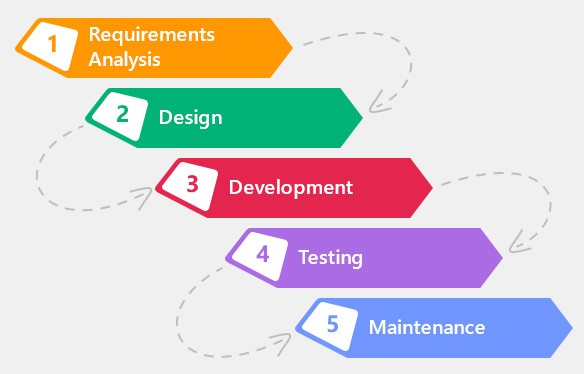
\includegraphics[width=\linewidth]{img/software-development-life-cycle.jpg}
		\caption{Lebenszyklus einer Software {\color{red}TODO: Replace with own diagram}}
		\label{fig:software-development-life-cycle}
	\end{wrapfigure}
	
	In vielen Modellen über den Lebenszyklus einer Software gibt es eine Phase, in der Instandhaltung und Support den Alltag bestimmen, sie wird oftmals ``Maintenance`` bezeichnet \cite{ManagingTheComplexityOfWebSystemsDevelopment} \cite{CostBenefitAnalaysisHumanFactorsSoftwareLifecycle}. Sie ist nach Zelkowitz \etal \cite{PrinciplesOfSoftwareEngineeringAndDesign} für rund zwei Drittel der Entwicklungskosten verantwortlich, begründet durch exponentielle Steigung \cite{ExtremeProgrammingExplained}.
	
	Es werden immer bessere Methoden entwickelt, um Probleme in Software - oder auch Bugs - zu verringern. Jedoch erhöht sich zugleich die Komplexität von Software, was zur Ursache hat, dass es mehr Nährboden für Bugs gibt \cite{TrackingDownSoftwareBugsAnomalyDetection}. De-facto sind Bugs ein unvermeidbarer Bestandteil einer Software und müssen daher erwartet und gehandhabt werden \cite{TheMythicalManMonth}.
	
	Wenn nun ein Bug auffällt, sei es durch einen Nutzer oder auch zufällig einem Stakeholder, muss entschieden werden, ob dieser zu beheben ist. Wenn eine Behebung angestrebt wird, benötigt der Stakeholder meistens Rahmeninformationen \citationneeded um den Bug ggf. zu reproduzieren und die Situation \textbf{nachzuvollziehen}. Desto mehr Verständnis der Stakeholder über das Problem erhält, desto schneller und präziser kann er die Ursache aufdecken. Die Ermöglichung der schnellen Verständnis über ein Problem, wird in dieser Arbeit Nachvollziehbarkeit genannt.

\section{Nachvollziehbarkeit}

	Sie beschäftigt sich mit der Informationserfassung und -aufbereitung, um das Verhalten eines Systems und die Interaktionen der Nutzer verstehen zu können.

\section{Maintenance bei Webapplikationen}

	\textit{Hier sollen die Besonderen Hürden bei Webapplikationen hervorgehoben werden (ungeschulte Nutzer, indirekte Kommunikation, etc.)}